%------------------------------------------------
\begin{frame}
\frametitle{The malposition and it's effects}
\hypertarget{malposition}{}
\begin{columns}[c] % The "c" option specifies centered vertical alignment while the "t" option is used for top vertical alignment

\column{.5\textwidth} % Left column and width

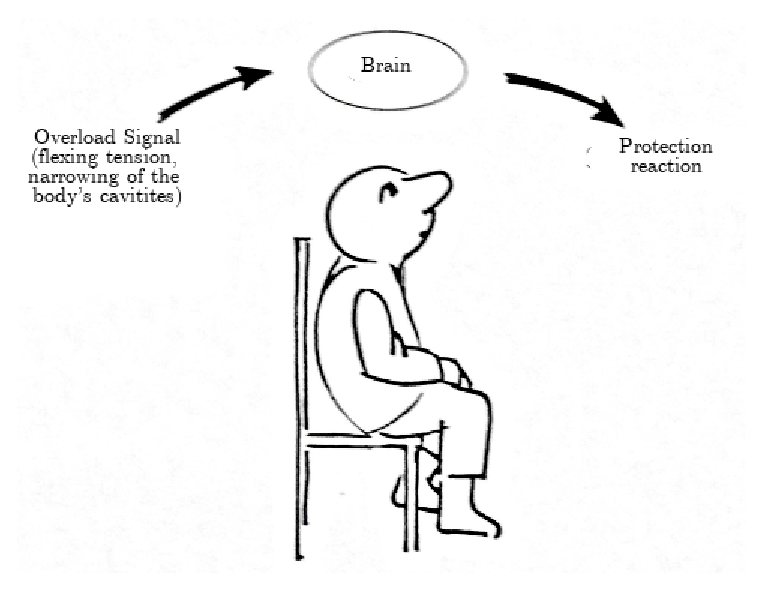
\includegraphics[width=1.1\linewidth]{Sitting_guy}

\column{.4\textwidth} % Left column and width
It's not only the \structure{skeleton} which experiences a strain in a malposition, also the \structure{visceral cavity} gets affected negatively. The \structure{pressure} which we seemingly are exposed to, puts pressure on our \structure{psyche and mood}.


\end{columns}
The strain of the malposition leads to a \structure{mechanical strain} of the \structure{musculoskeletal system}. This strain significantly \structure{reduces the mechanical load capacity}. This leads our body to react with \structure{protective measures} to counteract that strain.


\end{frame}
%------------------------------------------------

\begin{frame}
\frametitle{The malposition and it's effects II}
\begin{columns}[c] % The "c" option specifies centered vertical alignment while the "t" option is used for top vertical alignment

\column{.3\textwidth} % Left column and width

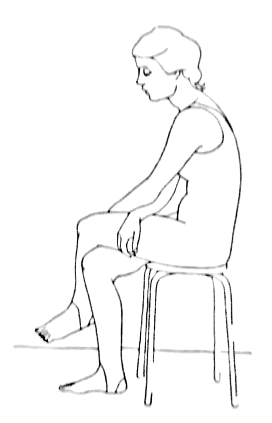
\includegraphics[width=1.1\linewidth]{Sitting_posture_Bad}

\column{.7\textwidth} % Left column and width
Only the physiological posture grants \structure{optimal spatial conditions} in the visceral cavity. Every curvature of the spine \structure{contracts the organs} of the chest and the belly region. A \structure{physical evasion} is possible, but severely \structure{impairs the function} of the organs.

Every single human makes between \structure{15,000 and 30,000 breaths every day}. Over weeks and months, even the smallest \structure{errors accumulate} and will lead to tangible consequences. A bad posture with \structure{tense abdominal muscles} and \structure{inhibited diaphragm} or then \structure{caved in shoulders} with \structure{constricted visceral cavity} (often all of that) will inhibit up to 30,000 times daily the breath.
\end{columns}


\end{frame}
%------------------------------------------------
%------------------------------------------------

\begin{frame}
\frametitle{The malposition and it's effects III}
\begin{columns}[c] % The "c" option specifies centered vertical alignment while the "t" option is used for top vertical alignment

\column{.3\textwidth} % Left column and width

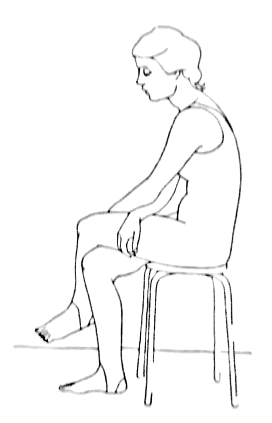
\includegraphics[width=1.1\linewidth]{Sitting_posture_Bad}

\column{.7\textwidth} % Left column and width
In a malposition, our \structure{vestibular} comes into a \structure{zone of depression}. A physiological posture is necessary for an optimal state of the psyche. 

A malposition leads to \structure{unnecessary tension and pressure} in our body. This leads to our body constantly being in a \structure{fight}. This will affect our \structure{thinking patterns}. Fights never lead to peace. Without peace, our progress will be stunted.
\end{columns}


\end{frame}
%------------------------------------------------